\documentclass[12pt]{article}
\usepackage[top=1cm, bottom=3cm, right=2cm, left=2cm]{geometry}
\usepackage{amsfonts, amssymb, amsmath, hyperref}
\usepackage{graphicx}
\usepackage[T1, T2A]{fontenc} % T2A for Cyrillic font encoding
\usepackage[english, russian]{babel}
\usepackage[justification=centering]{caption}
\usepackage{wrapfig,lipsum,booktabs}
\usepackage{placeins}
\usepackage{subcaption}
\usepackage{multirow}
\usepackage{indentfirst}
% \usepackage{lmodern} % Add this line to use the Latin Modern font

\begin{document}
\title{\textbf{Лабораторная работа 4.3.2}\\ [2pt]{Дифракция света на ультразвуковой волне в жидкости}}
\date{\today}
\author{Татаурова Юлия, Павлов Матвей}

\begin{document}
\maketitle
\section*{Аннотация}
В работе мы 
\section*{Теоретические сведения}

\indent При прохождении ультразвуковой (УЗ) волны через жидкость в ней возникают периодические оптические неоднородности, обусловленные разницей значений коэффициента преломления в областях сжатия и разрежения. Эти периодические неоднородности играют роль своеобразной дифракционной решётки для проходящего сквозь жидкость света.\\

\indent
Пусть УЗ-волна распространяется вдоль оси $X$ в жидкости, налитой в стеклянную кювету. В направлении оси $Z$ сквозь жидкость проходит световая волна, испытывающая дифракцию на акустической решётке. Поскольку скорость света значительно больше скорости звука, акустическую решётку можно считать неподвижной. Вызванное ультразвуком возмущение показателя преломления жидкости в нашем случае очень мало. При этом естественно сделать предположение, что акустическую решётку можно рассматривать как тонкий фазовый экран.

При небольших амплитудах звуковой волны показатель преломления жидкости $n$ меняется по закону:
\begin{equation}
n = n_0(1 + m \cos\Omega x),
\end{equation}

\indent
Пусть фаза световых колебаний на передней поверхности жидкости равна нулю. Тогда на задней поверхности она равна
$$
\varphi = knL = \varphi_0(1 + m\cos\Omega x),
$$
где $L$ — толщина слоя жидкости в кювете, $\varphi_0=kn_0L$. Таким образом, в плоскости $z=0$ фаза световых колебаний является периодической функцией координаты $x$, иными словами — УЗ-волна в жидкости создаёт фазовую дифракционную решётку.\\

\indent
Можно сформулировать качественный критерий, при выполнении которого можно считать акустическую решётку чисто фазовой, т.е. рассматривать её как тонкий фазовый экран. Для нашей задачи условие тонкого транспаранта можно записать в виде:
$$
m \ll \frac{\Lambda}{L} \sqrt{\frac{\lambda}{L}}.
$$
\indent
Таким образом, чисто фазовая акустическая решётка реализуется лишь на достаточно слабой УЗ-волне. При повышении мощности ультразвука акустическая волна начинает работать как сложная амплитудно-фазовая решётка.\\

\indent
При малой глубине фазовой модуляции поле, после прохождения через кювету, будет представлять собой совокупность трёх волн:
\begin{equation}
f_0(x) = e^{im\cos \Omega x} \approx 1 + im\cos \Omega x = 1 + \frac{im}{2}e^{i\Omega x} + \frac{im}{2}e^{-i\Omega x}
\end{equation}


\indent
В методе тёмного поля вместо фазовой пластинки в $\pi/4$ фурье-плоскости на оптической оси устанавливается непрозрачный экран. Осевая плоская волна, фокусируясь линзой в начале координат фурье-плоскости, поглощается непрозрачным экраном и не участвует в формировании изображения. Боковые же волны остаются без изменения. Поле в выходной плоскости в этом случае имеет вид:
$$
f(x) = \frac{im}{2} e^{i\Omega x} + \frac{im}{2} e^{-i\Omega x} = im \cos \Omega x,
$$
а картина интенсивности:
$$
I(x) = m^2 \cos^2 \Omega x.
$$

\indent
Однако, в общем случае (когда глубина модуляции не является малой величиной) после прохождения через кювету световое поле представляет совокупность не трёх, а большого числа плоских волн, распространяющихся под углами, определяемыми условием
\begin{equation}
\Lambda \sin\theta_m = m\lambda \quad (m = 0, \pm 1, \pm 2, \ldots). \label{eq:difraction}
\end{equation}
Каждая из этих волн соответствует одному из максимумов в дифракционной картине Фраунгофера.

Определяя на опыте положение дифракционных максимумов различного порядка, можно найти длину $\Lambda$ УЗ-волны и вычислить скорость $v$ распространения ультразвуковых волн в жидкости, если известна частота $\nu$ колебаний кварцевого излучателя:
$$
v = \Lambda \nu.
$$
Длина $\Lambda$ ультразвуковой волны определяется с помощью \ref{eq:difraction}; в силу малости углов $\theta_m$ окончательное выражение может быть представлено в виде:

\begin{equation}
    l_m = mf \frac{\lambda}{\Lambda}\label{eq:l_m}
\end{equation}
\noindent
где $l_m$ — измеренное на опыте линейное расстояние между $m$-м и нулевым максимумами, а $f$ — фокусное расстояние объектива $O_2$.

\section*{Экспериментальная установка}

\textit{\textbf{Оборудование:} оптическая скамья, осветитель, два длин-
нофокусных объектива, кювета с жидкостью, кварцевый излучатель
с микрометрическим винтом, генератор ультразвуковой частоты, линза, вертикальная нить на рейтере, микроскоп.}\\

\textit{\textbf{Параметры Экспериментальной установки:}}\\
\textit{Цена деления микрометрического винта: 4 мкм}\\
\textit{Длина волны красного светофильтра: $\lambda_{\text{кр}} = 640 \pm 20$ нм}\\
\textit{Длина волны зеленого светофильтра: $\lambda_{\text{зел}} = 546 \pm 50$ нм}\\
\textit{Фокусное расстояние линзы: $F = 30$ cм}\\


\subsection*{I. Определение скорости ультразвука по дифракционной картине}
\begin{figure}[h!]
    \centering
    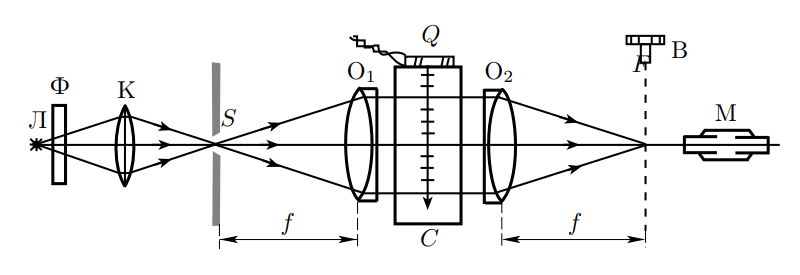
\includegraphics[width=0.8\linewidth]{images/setup1.png}
    \caption{Экспериментальная установка для наблюдения дифрации на акустической решётке}
    \label{fig:setup1}
\end{figure}

\indent
Источник света Л через светофильтр Ф и конденсор К освещает щель $S$, которая расположена в фокусе объектива $O_1$. Выходящий из объектива параллельный пучок света проходит через кювету $C$ перпендикулярно направлению распространения УЗ-волн. Эти волны возбуждаются в жидкости пьезокварцевой пластинкой $Q$, прикреплённой к стенке кюветы. На кварцевую пластинку подаётся напряжение ультразвуковой частоты от генератора. В фокальной плоскости второго объектива $O_2$ образуется дифракционная картина, наблюдаемая при помощи микроскопа $M$. \\\indent
Длина $\Lambda$ ультразвуковой волны определяется с помощью \ref{eq:difraction}; в силу малости углов $\theta_m$ окончательное выражение может быть представлено в виде
$$
l_m = mf\frac{\lambda}{\Lambda},
$$
Передвижением лизны была найдена чёткая дифракционная картинa.
% \begin{figure}[h!]
%     \centering
%     \includegraphics[width=8cm]{images/difr_image1.png}
%     \caption{Полученная дифракционная картина}
% \end{figure}


Затем, перемещая излучатель с помощью микрометрического винта, мы нашли расстояние между четкими дифракционными картинами и оценили по порядку величины
длину УЗ-волны как удвоенное расстояние между наиболее чёткими дифракционными картинами:
$
\Lambda = 2 \cdot 0.73 = 1.46 \text{ мм} \Rightarrow v_{\text{зв}} = \Lambda\nu = 1664 \text{ м/с}
$
\\\indent
Измерили положения $x_m$ пяти дифракционных максимумов для трех частот:

\begin{table}[h!]
    \centering
    \begin{tabular}{|c|c|c|c|}
        \hline
        $m / \nu$, \text{МГц} & 1.14 & 1.16 & 2.87\\\hline
        -2 &       6.14 & 6.6  & 5.56\\\hline
        -1 &       6.88 & 6.92 & 6.82\\\hline
         0 &       7.26 & 7.42 & 7.8 \\\hline
        +1 &       7.7  & 7.75 & 8.79\\\hline
        +2 &       8.2  & 8.17 & 9.75\\\hline
    \end{tabular}
    \caption{Зависимость расположения ($x_m$ мкм) дифракционных максимумов разных порядков от частоты}
\end{table}

\begin{figure}[h!]
    \centering
    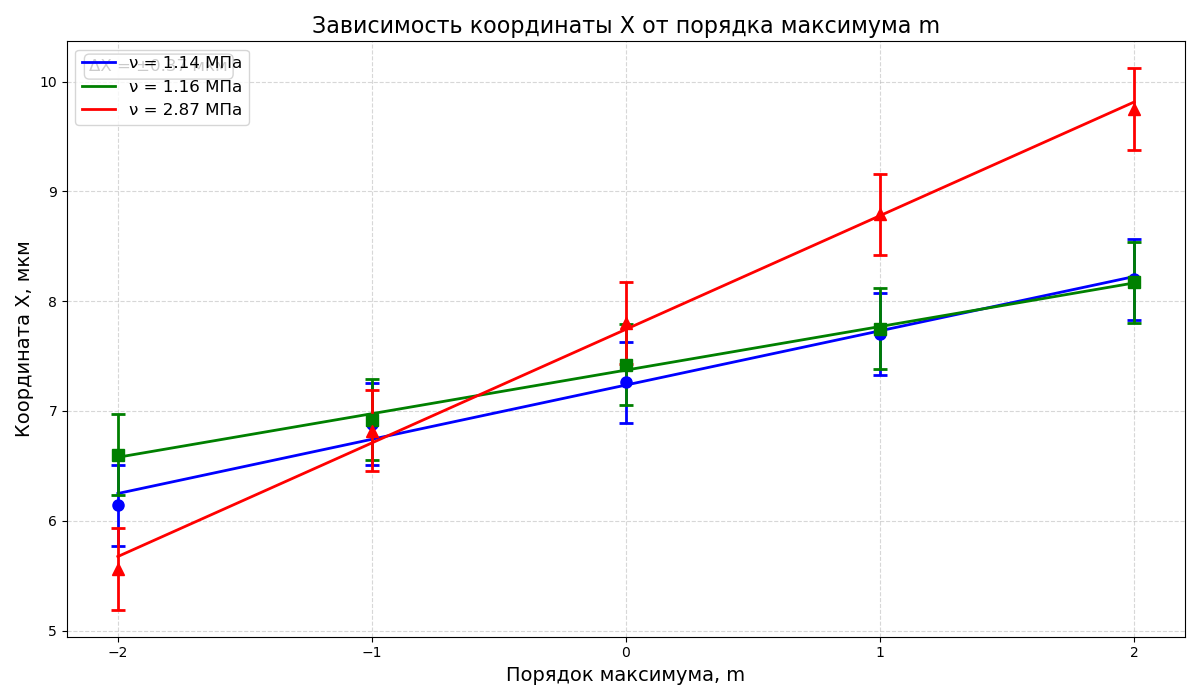
\includegraphics[width=18cm]{images/fig1.png}
\end{figure}

Расстояние между соседними  полосами вычислим по формуле:
\begin{equation}
    l = \frac{\Delta x_m}{\Delta m}
\end{equation}

По формуле \ref{eq:l_m} вычислим длину волны УЗ-волны. 
\begin{table}[h!]
    \centering
    \begin{tabular}{|c|c|c|c|}
        \hline
        \nu \text{, МГц} & 1.14 & 1.16 & 2.87 \\\hline
        l \text{, нм}    & 494 \pm 27 & 397 \pm 24 & 1035 \pm 31\\\hline
        \Lambda \text{, мм} & 3.7 \pm 0.2  & 4.8 \pm 0.3 & 1.8 \pm 0.1 \\\hline
        v \text{, м/с} & 4200 \pm 200 & 5560 \pm 350 & 5200 \pm 300\\\hline
    \end{tabular}
    \caption{Расстояние между соседними полосами и длина ультразвуковой волны для различных частот}
\end{table}

\subsection*{II. Определение скорости ультразвука методом тёмного поля}

\begin{figure}[h!]
    \centering
    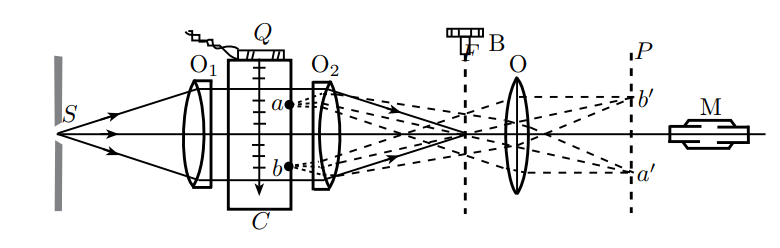
\includegraphics[width=0.8\linewidth]{images/setup2.png}
    \caption{Экспериментальная установка для наблюдения акустической решётки методом темного поля}
    \label{fig:setup2}
\end{figure}

Получили видимое изображение фазовой акустической решётки. Для этого, прежде всего, получилили в поле зрения микроскопа изображение задней плоскости кюветы. Это достигается с помощью вспомогательной положительной линзы $O$, которую располагают на оптической скамье за фокальной плоскостью объектива $O_2$.
\\\indent
Для наблюдения пространственной структуры фазовой решётки можно использовать метод\emph{тёмного поля}, основанный на устранении центрального дифракционного максимума с помощью специального экрана. \\\indent

В поле зрения микроскопа будут наблюдаться чередующиеся светлые и тёмные полосы, причём расстояние между тёмными полосами соответствует смещению в плоскости кюветы на $\Lambda/2$. Таким образом, должно наблюдаться характерное для метода тёмного поля удвоение числа деталей рассматриваемой структуры.

\\\indent
К задней стенке кюветы прижмали стеклянную пластинку с миллиметровыми делениями. Передвигая
микроскоп, сфокусировали его на изображение пластинки.
Определили цену деления окулярной шкалы в условиях опыта: \textbf{цена деления шкалы в микроскопе 0.1 мм}.

\\\indent
Закрыли центральный дифракционный максимум вертикальной нитью. Измерили длину УЗ-волны в воде. Для этого с помощью окулярной шкалы измерили расстояние между самыми дальними из хорошо видимых в поле зрения тёмных посчитайли число промежутков между ними.

При частоте $\nu = 1.14$ МГц число темных полос равно $n = 10$. При этом расстояние между полосами $\delta = 0.94$ мм. Тогда расстояние между полосами будет $l = \frac{\delta}{n} = 0.94 $ мм. Длина ултразвуковой волны $\Lambda = \frac{f\lambda}{l} = 2 \pm 0.4$ мм. Тогда скорость звука в воде $v = 2280 \pm 450$ м/с.

\section*{Вывод}
Мы получили длину УЗ-волны различными способами. Сначала по расстоянию между полосами дифракционной картины на акустической решетке. Результаты менялись в зависимости от частоты. Табличное знаение для длины УЗ-волны в воде порядка 1.5 мм. Мы получили разброс значений от 1.5 мм до почти 5 мм в зависимости от частоты генератора. Это можно обЪяснить тем, что в кювете могла быть и не вода вовсе или вода с примесями, поэтому значения могут варьироваться. Еще одной причиной может быть неточное определение координат полос и расстояний между ними, потому что мы могли ошибиться на полуширину этой полосы.


\end{document}
